\documentclass[11pt,aspectratio=169]{beamer}

\usetheme{Madrid}
\usecolortheme{seahorse}

\usepackage[utf8]{inputenc}
\usepackage{amsmath,amssymb}
\usepackage{xcolor}
\usepackage{booktabs}
\usepackage{tikz}
\usetikzlibrary{arrows.meta,positioning,fit,backgrounds}

\setbeamertemplate{navigation symbols}{}
\setbeamertemplate{footline}[frame number]

\title{Beyond the Syllabus}
\subtitle{Union-Find and Graph Connectivity: Provable Limits, Concurrent Algorithms,
and Planet-Scale Systems\\
\small Week 3 Supplement -- TOAE209/TOAH209: Design and Analysis of Algorithms}
\author{Foreign Trade University}
\date{}

\begin{document}

% ---------------------------------------------------------------
\begin{frame}
  \titlepage
\end{frame}
% ---------------------------------------------------------------

\begin{frame}{Outline}
  \tableofcontents
\end{frame}

% =================================================================
\section{Motivation}
% =================================================================

\begin{frame}{Why look beyond the syllabus?}
  \begin{itemize}
    \item This week you proved that Union-Find, with union by rank and path
    compression, costs $O(m\,\alpha(n))$ total time for $m$ operations -- essentially
    constant per operation. You also traced BFS and DFS, both $O(n+m)$.
    \item Four questions a curious student should ask next -- each one turns out to be
    an active (or very recently settled) research question:
    \begin{enumerate}
      \item Is $O(m\,\alpha(n))$ actually the \textbf{best possible}, or could a
      smarter data structure beat it?
      \item Union-Find only handles edges being \textbf{added}. What if edges can also
      be \textbf{deleted}?
      \item What happens if \textbf{many threads} call \texttt{union} at the same
      time?
      \item Your BFS/DFS ran on a graph with a few hundred vertices. What does it take
      to run the \textbf{same idea} on a graph with \textbf{128 billion edges}?
    \end{enumerate}
  \end{itemize}
  \begin{alertblock}{How this supplement is different from a survey}
    Every section below walks through the \emph{actual mechanics} of an algorithm --
    with a hand-traceable running example -- not just a headline result. Where I quote
    a specific bound or number, it is sourced to a specific paper (cited on the slide).
  \end{alertblock}
\end{frame}

% =================================================================
\section{Closing the Loop: Is Union-Find Provably Optimal?}
% =================================================================

\begin{frame}{Recap: the bound you proved this week}
  \begin{block}{Theorem (this week's lecture notes)}
    With union by rank \emph{and} path compression, a sequence of $m$
    \texttt{find}/\texttt{union} operations on $n$ elements takes $O(m\,\alpha(n))$
    total time, where $\alpha$ is the inverse Ackermann function.
  \end{block}
  \begin{itemize}
    \item This is an \textbf{upper bound}: a guarantee that this particular algorithm
    (rank $+$ compression) never does worse.
    \item It says nothing about whether some entirely different data structure --
    with a cleverer invariant, more bits of state per element, anything -- could do
    \emph{better}. Ruling that out requires a completely different kind of argument:
    a \textbf{lower bound} that applies to \emph{every} possible algorithm.
    \item Fredman and Saks (STOC 1989, ``The Cell Probe Complexity of Dynamic Data
    Structures'') proved exactly such a lower bound, 14 years after Tarjan's 1975
    upper bound. \emph{DOI:} \texttt{10.1145/73007.73040}.
  \end{itemize}
\end{frame}

\begin{frame}{Just how slowly does $\alpha(n)$ actually grow?}
  \small
  Before the lower bound, get a feel for the function being bounded. Recall
  $\log^* n$ (``iterated log''): the number of times you apply $\log_2$ before the
  result drops to $\le 1$. $\alpha(n)$ grows even \emph{slower} than $\log^* n$.
  \begin{center}
  \begin{tabular}{@{}lccccc@{}}
    \toprule
    $n$ & step 1 & step 2 & step 3 & step 4 & $\log^* n$ \\
    \midrule
    $2$ & $1$ & -- & -- & -- & $1$ \\
    $4$ & $2$ & $1$ & -- & -- & $2$ \\
    $16$ & $4$ & $2$ & $1$ & -- & $3$ \\
    $65{,}536$ & $16$ & $4$ & $2$ & $1$ & $4$ \\
    $2^{65536}$ (a $19{,}729$-digit number) & $65{,}536$ & $16$ & $4$ & $2\to1$ & $5$ \\
    \bottomrule
  \end{tabular}
  \end{center}
  \begin{exampleblock}{Hand-checkable}
    $\log_2 65536 = 16$, $\log_2 16 = 4$, $\log_2 4 = 2$, $\log_2 2 = 1$: four steps, so
    $\log^*(65536)=4$. And $2^{65536}$ has about $19{,}729$ decimal digits -- far more
    than the $\sim 10^{80}$ atoms in the observable universe -- yet needs only \emph{one
    more} step: $\log^*(2^{65536}) = 5$. No $n$ you could ever write down needs
    $\log^* n > 5$, and $\alpha(n)$ is even flatter than this.
  \end{exampleblock}
\end{frame}

\begin{frame}{The lower bound: proof idea (Fredman--Saks, 1989)}
  \small
  \textbf{Model:} the \emph{cell-probe} model -- charge an algorithm only for memory
  \emph{words read or written}, ignoring all local computation (the most generous
  possible model for an algorithm to work in, so a lower bound here is very strong).
  \begin{itemize}
    \item \textbf{Adversary construction.} Build a specific, structured sequence of
    $m$ interleaved \texttt{union}/\texttt{find} calls on $n$ elements, organized into
    \textbf{epochs}, where each epoch forces some \texttt{find} to depend on
    information written many epochs earlier.
    \item \textbf{Counting argument.} Few memory probes per \texttt{find} means little
    information can flow between far-apart epochs -- but the adversary sequence needs
    a specific number of ``surviving'' epochs to avoid contradiction, and that number
    grows like the inverse Ackermann function.
    \item \textbf{Conclusion:} \emph{any} algorithm (not just rank $+$ compression)
    must spend $\Omega(m\,\alpha(n))$ total cell probes on some such sequence.
  \end{itemize}
  \begin{exampleblock}{Why only a sketch}
    The full ``chronogram technique'' proof is one of the most technically involved
    lower bounds in data structures -- normally only sketched even in graduate
    courses. Take away \emph{what kind of argument} proves a lower bound (adversary
    $+$ information counting), a different skill from proving an upper bound.
  \end{exampleblock}
\end{frame}

\begin{frame}{The lesson: a 14-year-old gap, closed}
  \begin{center}
  \begin{tabular}{@{}lll@{}}
    \toprule
    Year & Result & What it establishes \\
    \midrule
    1975 & Tarjan (upper bound) & $O(m\,\alpha(n))$ suffices \\
    1984 & Tarjan \& van Leeuwen (refinement) & tight analysis of rank $+$ compression \\
    1989 & Fredman \& Saks (lower bound) & $\Omega(m\,\alpha(n))$ is \emph{necessary} \\
    \bottomrule
  \end{tabular}
  \end{center}
  \begin{alertblock}{The takeaway}
    The algorithm you hand-traced this week is not a good-enough approximation of some
    better algorithm nobody has found yet. It is, up to constant factors, \textbf{the
    fastest possible} amortized Union-Find in this model -- full stop. That is a rare
    and satisfying thing to be able to say about an algorithm you can implement in 20
    lines of code.
  \end{alertblock}
\end{frame}

% =================================================================
\section{What If Edges Can Also Disappear? Fully Dynamic Connectivity}
% =================================================================

\begin{frame}{The limitation: Union-Find only grows}
  \begin{itemize}
    \item Everything this week assumed edges are only ever \textbf{added}. That is
    exactly the right model for Kruskal's MST (a later week) -- but real networks lose
    edges too: a road closes, a link goes down, a friendship ends.
    \item \textbf{Question:} can we maintain ``are $u$ and $v$ connected?'' under both
    edge insertions \emph{and} deletions, still faster than recomputing from scratch?
  \end{itemize}
  \begin{block}{The naive baseline}
    After every deletion, rerun BFS/DFS from scratch: $O(n+m)$ per update. For a graph
    with millions of updates (a live social graph, a router table), this is far too
    slow -- we want something closer to Union-Find's near-constant cost, in both
    directions.
  \end{block}
  \begin{exampleblock}{Why Union-Find itself can't be patched}
    Union-Find has no memory of \emph{why} two elements got connected -- once you
    union$(x,y)$, the specific edge is forgotten. Deleting ``the edge that caused the
    union'' is meaningless to the data structure: there is no way back.
  \end{exampleblock}
\end{frame}

\begin{frame}{The key idea: give every edge a \emph{level}}
  Holm, de Lichtenberg, and Thorup (\textbf{HDT}, J.\ ACM 2001) maintain a spanning
  forest $F$ where every tree edge $e$ carries a level $\ell(e) \in \{0,\dots,L\}$,
  $L = \lceil \log_2 n \rceil$.
  \begin{block}{The level invariant}
    Let $F_i = \{e \in F : \ell(e) \ge i\}$, so $F = F_0 \supseteq F_1 \supseteq \dots
    \supseteq F_L$. Invariant: every tree of $F_i$ has \textbf{at most $n/2^i$
    vertices}. New edges always start at level $0$.
  \end{block}
  \begin{itemize}
    \item Each level's forest $F_i$ is stored in an \textbf{Euler-tour tree}: a
    balanced structure supporting \texttt{link}, \texttt{cut}, \texttt{find-root}, and
    \texttt{subtree-size}, all in $O(\log n)$ -- and (with extra bookkeeping) it can
    also report ``some non-tree edge touching this subtree'' in $O(\log n)$ amortized.
    \item Non-tree edges are stored per level too, indexed by their endpoints, so we can
    ask ``does any level-$i$ non-tree edge leave this subtree?''
  \end{itemize}
\end{frame}

\begin{frame}{Deleting a tree edge: the replacement-edge search}
  \begin{block}{Algorithm: \textsc{Delete}$(e)$, where $e$ is a tree edge at level $i=\ell(e)$}
    \begin{enumerate}
      \item Cut $e$ from the Euler-tour trees at levels $0,1,\dots,i$ -- this splits
      one tree into two pieces, call them $T_1, T_2$.
      \item For level $j = i$ down to $0$:
      \begin{enumerate}
        \item Let $T_{\text{small}}$ be the smaller of $T_1 \cap F_j$, $T_2 \cap F_j$
        (found via an $O(\log n)$ size query).
        \item \textbf{Promote} every tree edge inside $T_{\text{small}}$ from level $j$
        to level $j+1$ (this is safe: $T_\text{small}$ has $\le n/2^{j+1}$ vertices).
        \item Scan the non-tree edges touching $T_\text{small}$ at level $j$, one at a
        time. For each edge $(x,y)$:
        \begin{itemize}
          \item if $y \notin T_\text{small}$ (it reaches the \emph{other} piece):
          \textbf{replacement found} -- link it as a tree edge at level $j$. Stop.
          \item else ($y \in T_\text{small}$, a ``dud''): promote it to level $j+1$
          too, and keep scanning.
        \end{itemize}
      \end{enumerate}
      \item If level $0$ is exhausted with no replacement: the deletion genuinely
      increased the number of connected components.
    \end{enumerate}
  \end{block}
\end{frame}

\begin{frame}{Running example: deleting a bridge edge}
  \begin{columns}
  \begin{column}{0.46\textwidth}
  \begin{center}
  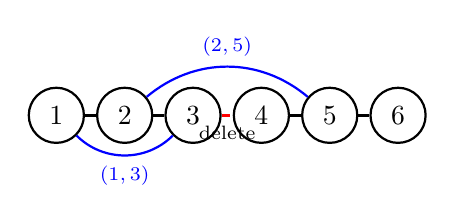
\begin{tikzpicture}[
      node distance=1cm,
      vtx/.style={circle, draw, thick, minimum size=7mm},
      >=Stealth]
    \foreach \i/\x in {1/0,2/1.4,3/2.8,4/4.2,5/5.6,6/7.0}
      \node[vtx] (v\i) at (\x*0.62,0) {\i};
    \draw[very thick] (v1)--(v2);
    \draw[very thick] (v2)--(v3);
    \draw[very thick, red, dashed] (v3)--(v4)
      node[midway, below, font=\scriptsize, black] {delete};
    \draw[very thick] (v4)--(v5);
    \draw[very thick] (v5)--(v6);
    \draw[thick, blue, bend left=40] (v2) to node[above,font=\scriptsize]{$(2,5)$} (v5);
    \draw[thick, blue, bend right=45] (v1) to node[below,font=\scriptsize]{$(1,3)$} (v3);
  \end{tikzpicture}
  \\[4pt]
  {\scriptsize solid = tree edges (level 0); blue = non-tree edges (level 0)}
  \end{center}
  \end{column}
  \begin{column}{0.54\textwidth}
  \small
  Delete tree edge $(3,4)$, level $i=0$. Splits $\{1,2,3\}$ vs.\ $\{4,5,6\}$ (tie,
  either could be $T_\text{small}$; take $\{1,2,3\}$).
  \begin{enumerate}
    \item Promote $(1,2)$ and $(2,3)$ to level $1$ (still tree edges, now also in
    $F_1$; $|\{1,2,3\}| = 3 \le n/2^1 = 3$ \checkmark).
    \item Scan non-tree edges touching $\{1,2,3\}$: first $(1,3)$ -- both endpoints
    inside $T_\text{small}$, a \textbf{dud}, promote to level $1$.
    \item Next $(2,5)$ -- endpoint $5$ is in the \emph{other} piece: \textbf{replacement
    found}. Link $(2,5)$ as a tree edge at level $0$.
  \end{enumerate}
  \end{column}
  \end{columns}
  \vspace{4pt}
  \begin{exampleblock}{Result}
    New spanning tree: $(1,2)_{L1}, (2,3)_{L1}, (2,5)_{L0}, (4,5)_{L0}, (5,6)_{L0}$ --
    all six vertices reconnected, and two edges are now ``used up'' at level $1$ where
    they can help future, smaller-scale searches.
  \end{exampleblock}
\end{frame}

\begin{frame}{Why this is fast: the amortized argument}
  \begin{itemize}
    \item There are only $L = O(\log n)$ levels, and each edge's level only ever
    \textbf{increases} -- so any single edge can be promoted at most $O(\log n)$ times
    over its entire lifetime.
    \item Charge each promotion to the edge being promoted: total promotion work over
    the \emph{whole} sequence of $m$ operations is $O(m \log n)$, i.e.\ $O(\log n)$
    \textbf{amortized} per operation.
    \item Each \texttt{Delete} also does $O(\log n)$ levels of ``search,'' each costing
    $O(\log n)$ for the Euler-tour-tree operations -- an extra $O(\log^2 n)$
    worst-case-looking cost, but the search that finds a replacement (or exhausts a
    level) is exactly what triggers the promotions that pay for it.
    \item Net result: $O(\log^2 n)$ \textbf{amortized} time per update, $O(\log n /
    \log\log n)$ per connectivity query, with a refinement -- Holm, de Lichtenberg,
    Thorup, J.\ ACM 2001.
  \end{itemize}
\end{frame}

\begin{frame}{The race for \emph{worst-case} (not just amortized) bounds}
  \small
  HDT's $O(\log^2 n)$ is \emph{amortized}: one single update could still be slow, as
  long as the average stays low. Getting the \emph{same} guarantee on \textbf{every
  single} update turned into its own 25-year research program:
  \begin{center}
  \begin{tabular}{@{}lll@{}}
    \toprule
    Year & Result & Bound \\
    \midrule
    2001 & Holm, de Lichtenberg, Thorup & $O(\log^2 n)$ amortized \\
    2013 & Kapron, King, Mountjoy (SODA best paper) & polylog \emph{worst-case}, randomized \\
    2017 & Nanongkai, Saranurak, Wulff-Nilsen (FOCS) & $n^{o(1)}$ worst-case, Las Vegas \\
    2023--24 & Goranci, Henzinger, Nanongkai, Saranurak, & $\tilde O(n)$ worst-case, exact \\
             & Thorup, Wulff-Nilsen & \emph{edge connectivity} \\
    2024 & Jin, Sun, Thorup (SODA) & dynamic min-cut, subpolynomial \\
    \bottomrule
  \end{tabular}
  \end{center}
  \begin{alertblock}{An open question, resolved -- this decade}
    The 2023--24 result answers, in the affirmative, a question Thorup himself posed
    in \emph{Combinatorica}, 2007: can \emph{exact edge connectivity} (not just
    yes/no reachability) be maintained with worst-case $o(m)$ update time? As of this
    month (August 2026), arXiv preprints (e.g.\ 2510.08297, 2605.15173, 2601.20137)
    show the bounds are \textbf{still being pushed further, right now}.
  \end{alertblock}
\end{frame}

% =================================================================
\section{One Structure, Many Threads: Concurrent Union-Find}
% =================================================================

\begin{frame}{The problem: Union-Find was never designed for parallel hardware}
  \begin{itemize}
    \item Modern CPUs have dozens of cores; GPUs have thousands. Computing connected
    components of a huge graph means many threads calling \texttt{union} and
    \texttt{find} \emph{at the same time}, on the \emph{same} \texttt{parent[]} array.
    \item The sequential algorithm from this week is \textbf{not safe} under
    concurrency -- two threads racing on the same memory can corrupt the structure.
  \end{itemize}
  \begin{exampleblock}{A concrete race: a cycle appears}
    $x,y$ start as singleton roots. Thread $A$ runs \texttt{union}$(x,y)$; Thread $B$
    runs \texttt{union}$(y,x)$, at the same instant.
    \begin{enumerate}
      \item Both threads read $root(x)=x$ and $root(y)=y$ \emph{before either writes}.
      \item $A$ decides to set $parent[x] \gets y$; $B$ decides to set $parent[y]
      \gets x$ -- based on stale information.
      \item Both writes go through: $parent[x]=y$ \textbf{and} $parent[y]=x$. Now
      \texttt{find}$(x)$ loops \textbf{forever}. The tree invariant is destroyed.
    \end{enumerate}
  \end{exampleblock}
\end{frame}

\begin{frame}{The fix: compare-and-swap, plus a tie-break rule}
  \begin{block}{\textsc{CAS-Union}$(x,y)$}
  \begin{enumerate}
    \item \textbf{loop:}\ $r_x \gets \textsc{Find}(x)$;\ $r_y \gets \textsc{Find}(y)$
    \item if $r_x = r_y$: return (already unioned)
    \item if $r_x < r_y$: swap$(r_x, r_y)$ \hfill \small\emph{-- fixed, deterministic tie-break}
    \item if $\text{CAS}(parent[r_x],\, r_x,\, r_y)$ succeeds: return
    \item else: \textbf{retry} the whole loop (someone else moved $r_x$ concurrently)
  \end{enumerate}
  \end{block}
  \begin{block}{\textsc{Find}$(x)$ -- with best-effort path halving}
  \begin{enumerate}
    \item while $parent[x] \ne x$: let $p \gets parent[x]$;\ attempt
    $\text{CAS}(parent[x], p, parent[p])$ (ok if it fails -- just an optimization);\
    $x \gets p$
    \item return $x$
  \end{enumerate}
  \end{block}
\end{frame}

\begin{frame}{Why this fixes the race}
  \begin{exampleblock}{Two ideas doing the real work}
    \begin{itemize}
      \item The \textbf{deterministic tie-break} (\emph{always} attach the smaller
      root under the larger, regardless of which thread got there first) rules out
      the two-writer cycle from the previous slide \emph{by construction} -- both
      threads, no matter what they observe, agree on which direction the edge must
      point.
      \item The \textbf{CAS-and-retry loop} means a losing thread \emph{notices} it
      lost (its compare-and-swap fails because $parent[r_x]$ no longer matches what
      it read) and safely recomputes, instead of overwriting blindly with stale
      information.
    \end{itemize}
  \end{exampleblock}
\end{frame}

\begin{frame}{Tracing the fix on the exact race that broke us}
  Same scenario: $A$ runs \texttt{union}$(x,y)$, $B$ runs \texttt{union}$(y,x)$,
  concurrently. Say $x < y$, so the tie-break always targets
  $parent[x] \gets y$, no matter which thread computes it.
  \begin{enumerate}
    \item Both $A$ and $B$ read $r_x = x,\ r_y = y$; both apply the \emph{same}
    tie-break rule and both attempt $\text{CAS}(parent[x],\, x,\, y)$.
    \item Say $A$'s CAS runs first: $parent[x]$ was $x$, so it succeeds --
    $parent[x] \gets y$. $A$ returns.
    \item $B$'s CAS now runs: it expects $parent[x]$ to still be $x$, but it is now
    $y$ -- \textbf{CAS fails}. $B$ retries: recomputes $r_x = \textsc{Find}(x) = y$,
    $r_y = \textsc{Find}(y) = y$. Now $r_x = r_y$: $B$ returns immediately.
  \end{enumerate}
  \begin{exampleblock}{No cycle, no lost update}
    Exactly one union happens; the loser detects the conflict and safely no-ops. This
    is the general pattern behind lock-free data structures: never overwrite blindly,
    always verify-then-commit, and retry on failure.
  \end{exampleblock}
\end{frame}

\begin{frame}{Jayanti and Tarjan (PODC 2016): making the guarantee rigorous}
  \small
  The CAS loop above is the accessible \emph{idea}. Proving a tight
  \emph{worst-case} time bound under an adversarial thread scheduler is much harder --
  solved by Sam Jayanti and \textbf{Robert Tarjan} (the same Tarjan behind this week's
  classical rank-and-compression analysis, four decades earlier).
  \begin{block}{The result}
    A deterministic \textbf{wait-free} algorithm (double-CAS), plus two randomized
    algorithms (ordinary CAS only), all achieve total work
    $O\big(m(\log(\tfrac{np}{m}+1) + \alpha(n,\tfrac{m}{np}))\big)$
    for $n$ elements, $m$ operations, $p$ concurrent processes -- essentially the
    \emph{same} inverse-Ackermann-type bound as the sequential algorithm, even under
    adversarial scheduling.
  \end{block}
  \begin{exampleblock}{Why it matters in practice}
    This style of algorithm is now, per the subsequent literature, the practical basis
    for the \textbf{fastest known} connected-components code on both CPUs and GPUs.
  \end{exampleblock}
\end{frame}

% =================================================================
\section{Union-Find and Traversal at Planetary Scale}
% =================================================================

\begin{frame}{From a homework graph to the entire Web}
  \begin{itemize}
    \item This week's BFS/DFS/Union-Find are all $O(n+m)$ -- instant on a graph with a
    few hundred vertices. What about the \textbf{Hyperlink2012} web graph: $3.5$
    \textbf{billion} vertices, $128$ \textbf{billion} edges?
  \end{itemize}
  \begin{block}{Dhulipala, Blelloch, Shun (SPAA 2018) -- the GBBS/Ligra system}
    Computing all connected components of Hyperlink2012 took \textbf{25.0 seconds}
    on a \emph{single} shared-memory machine with $72$ cores.
  \end{block}
  \begin{center}
  \begin{tabular}{@{}lll@{}}
    \toprule
    System & Hardware & Time \\
    \midrule
    GBBS/Ligra (2018) & 1 machine, 72 cores & \textbf{25.0 s} \\
    Distributed cluster (Stergiou et al.) & 1000 nodes, 12{,}000 cores, 128TB RAM & 341 s \\
    Supercomputer (Slota et al.) & $>8000$ cores & $\approx$ 6 min \\
    \bottomrule
  \end{tabular}
  \end{center}
  $13.6\times$ faster than the cluster, using $166\times$ fewer cores and $128\times$
  less memory. This work (Ligra/GBBS/Aspen) won the 2022 ACM Paris Kanellakis Theory
  and Practice Award.
\end{frame}

\begin{frame}{How? The same algorithm, engineered to be work-efficient in parallel}
  \begin{itemize}
    \item No new algorithmic idea is needed at the core: a \textbf{direction-optimizing
    BFS} (switch between expanding the frontier ``top-down'' from visited vertices, and
    ``bottom-up'' by checking unvisited vertices for a visited neighbor, whichever is
    cheaper for the current frontier size) combined with a \textbf{parallel-safe
    Union-Find} -- exactly the CAS-based \texttt{union} from the previous section,
    applied to all edges at once.
    \item Total work stays $O(n+m)$; what changes is that the work is spread across
    many cores with high memory locality and (nearly) no synchronization overhead --
    an \emph{engineering} achievement built directly on top of this week's algorithms
    and last section's concurrency result.
  \end{itemize}
\end{frame}

\begin{frame}{A sharper shortcut for real graphs: sampling (Afforest)}
  Real graphs (web, social networks) are \textbf{power-law}: a handful of hub vertices
  touch a huge share of all edges, and almost every vertex sits in one giant component.
  Sutton, Ben-Nun, and Barak (IPDPS 2018, \emph{``Optimizing Parallel Graph
  Connectivity Computation via Subgraph Sampling''}) exploit exactly this:
  \begin{block}{Afforest, three steps}
    \begin{enumerate}
      \item \textbf{Sample rounds:} for $2$ rounds, link every vertex to just
      \emph{one} neighbor (not all of them). On a power-law graph this alone merges
      almost everything into a few giant components.
      \item \textbf{Identify the giant component:} randomly sample $1024$ vertices;
      the most frequent component label among them is (almost certainly) the giant
      component.
      \item \textbf{Skip and finish:} scan all edges once, but \textbf{skip} any edge
      whose two endpoints are \emph{already} both known to be in the giant component --
      the vast majority of edges. Union the (few) remaining edges normally.
    \end{enumerate}
  \end{block}
  Same $O(n+m)$ worst case, but in practice most of the $m$ is never touched.
\end{frame}

\begin{frame}{FastCC (2026): one BFS, from the right vertex}
  \begin{itemize}
    \item ACM Transactions on Architecture and Code Optimization, 2026
    (\emph{DOI:} \texttt{10.1145/3803020}) pushes the power-law idea further:
    instead of random sampling rounds, \textbf{fix the BFS root at the single
    highest-degree vertex}, and run one BFS.
    \item On a power-law graph, that one BFS from the ``hub'' typically reaches
    almost the entire giant component in a single, predictable, well-load-balanced
    pass -- avoiding the irregular frontier sizes that make plain BFS slow and
    imbalanced on these graphs.
  \end{itemize}
  \begin{exampleblock}{Reported results}
    $10.6$--$55.5\times$ (average $37.8\times$) faster than prior state-of-the-art
    connected-components implementations (including systems built on the GBBS/Afforest
    ideas above), up to $2.87\times$ less peak memory -- and it is the engine behind a
    top-ranked \textbf{GreenGraph500} entry (a supercomputing benchmark ranked by
    \emph{energy efficiency}, not just raw speed).
  \end{exampleblock}
\end{frame}

\begin{frame}{The lesson}
  \begin{alertblock}{Same two primitives, all the way up}
    Every system in this section -- a homework BFS, a 72-core machine indexing the
    web, a 2026 energy-efficiency record -- is built from exactly the two ideas you
    hand-traced this week: \textbf{graph traversal} and \textbf{Union-Find}. What
    changes from a classroom exercise to a production system is not the algorithm's
    asymptotic bound, but decades (and counting) of work on making that same $O(n+m)$
    bound actually fast on real hardware and real, power-law-shaped data.
  \end{alertblock}
\end{frame}

% =================================================================
\section{Bonus: Topological Sort Is Quietly Running Your Software}
% =================================================================

\begin{frame}{Kahn's algorithm, everywhere}
  No new research needed here -- just naming where the exact algorithm from this
  week's notes (\textsc{Kahn}$(adj)$, Algorithm in Section 6) runs \textbf{today}:
  \begin{itemize}
    \item \texttt{pip}, \texttt{npm}, \texttt{cargo}: before installing anything, they
    topologically sort the package dependency DAG.
    \item \textbf{Bazel} / \textbf{Make}: build targets are scheduled in dependency
    order -- exactly Kahn's algorithm over the build graph.
    \item \textbf{PyTorch autograd} and \textbf{CUDA graph capture}: operations in a
    computation graph execute only after their inputs are ready -- a topological order
    of the op graph.
    \item \textbf{Airflow} DAGs and agent-orchestration frameworks (e.g.\ LangGraph):
    task nodes run only after their declared dependencies finish.
  \end{itemize}
\end{frame}

\begin{frame}{Worked example: resolving a package install order}
  \begin{columns}
  \begin{column}{0.42\textwidth}
  \begin{center}
  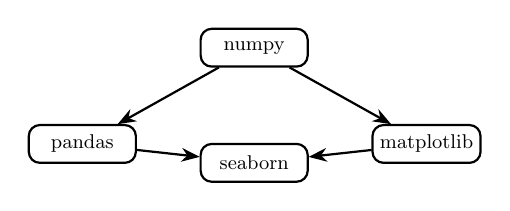
\begin{tikzpicture}[
      scale=0.8, every node/.style={transform shape},
      node distance=0.9cm and 1.0cm,
      pkg/.style={rectangle, draw, thick, rounded corners, minimum width=1.7cm,
      minimum height=0.6cm, font=\small},
      >=Stealth]
    \node[pkg] (np) {numpy};
    \node[pkg, below left=of np] (pd) {pandas};
    \node[pkg, below right=of np] (mp) {matplotlib};
    \node[pkg, below=1.2cm of np] (sb) {seaborn};
    \draw[->, thick] (np) -- (pd);
    \draw[->, thick] (np) -- (mp);
    \draw[->, thick] (pd) -- (sb);
    \draw[->, thick] (mp) -- (sb);
  \end{tikzpicture}
  \end{center}
  \end{column}
  \begin{column}{0.58\textwidth}
  \small
  In-degrees: $numpy{=}0$, $pandas{=}1$, $matplotlib{=}1$, $seaborn{=}2$.
  \begin{itemize}
    \item Queue $\gets [numpy]$ (only in-degree-0 vertex).
    \item Dequeue $numpy$; output it; decrement $pandas\to0$, $matplotlib\to0$; enqueue
    both.
    \item Dequeue $pandas$; output it; decrement $seaborn\to1$ (not yet $0$).
    \item Dequeue $matplotlib$; output it; decrement $seaborn\to0$; enqueue it.
    \item Dequeue $seaborn$; output it.
  \end{itemize}
  \end{column}
  \end{columns}
  \begin{exampleblock}{Result}
    \small Install order: $numpy \to pandas \to matplotlib \to seaborn$ (or $numpy \to
    matplotlib \to pandas \to seaborn$ -- both valid). This is \emph{literally}
    \textsc{Kahn}$(adj)$ from this week's notes, run on a dependency graph instead of
    a textbook example.
  \end{exampleblock}
\end{frame}

% =================================================================
\section{Summary}
% =================================================================

\begin{frame}{Summary}
  \small
  \begin{enumerate}
    \item \textbf{Provable optimality:} Fredman \& Saks (1989) proved Union-Find's
    $O(m\,\alpha(n))$ bound is not just good -- it is the best \emph{any} algorithm
    can do, in a very general model.
    \item \textbf{Deletions reopen everything:} allowing edges to disappear turns a
    20-line data structure into a 25-year (and still active) research program -- from
    $O(\log^2 n)$ amortized (2001) to worst-case results still being refined in 2026.
    \item \textbf{Concurrency needs its own proof:} a CAS-loop-with-tie-break fixes the
    obvious race, but Jayanti \& Tarjan (2016) needed a genuine research result to
    guarantee it under \emph{any} adversarial schedule -- now the practical backbone
    of real CPU/GPU connected-components code.
    \item \textbf{Scale is an engineering frontier, not a new algorithm:} this week's
    exact $O(n+m)$ ideas, tuned for real hardware and power-law graphs, index a
    128-billion-edge web graph in 25 seconds -- and a 2026 paper is still improving it.
  \end{enumerate}
  \begin{alertblock}{Looking ahead}
    Next week (Kleinberg \& Tardos, Chapter 4) reuses BFS as a stepping stone toward
    \textbf{greedy algorithms}, and Union-Find reappears as the core data structure
    behind Kruskal's Minimum Spanning Tree algorithm.
  \end{alertblock}
\end{frame}

\end{document}
